\documentclass[11pt]{scrartcl}
\usepackage[sexy]{evan}
\usepackage{graphicx}

\usepackage{answers}
\Newassociation{hint}{hintitem}{all-hints}
\renewcommand{\solutionextension}{out}
\renewenvironment{hintitem}[1]{\item[\bfseries #1.]}{}
\declaretheorem[style=thmbluebox,name={Theorem}]{thm}

 %Sets
\newcommand{\N}{\mathbb{N}}
\newcommand{\Z}{\mathbb{Z}}
\newcommand{\F}{\mathbb{F}}
\newcommand{\Q}{\mathbb{Q}}
\newcommand{\R}{\mathbb{R}}
\newcommand{\C}{\mathbb C}
\newcommand{\T}{\mathbb T}

\let \phi \varphi

%From Topology
\newcommand{\cT}{\mathcal{T}}
\newcommand{\cB}{\mathcal{B}}
\newcommand{\cC}{\mathcal{C}}
\newcommand{\cH}{\mathcal{H}}



\begin{document}
\title{Math 222a}
\author{Vishal Raman}
\thispagestyle{empty}
$ $
\vfill
\begin{center}

\centerline{\huge \textbf{Math 222a Lecture Notes, Fall 2020}}
\centerline{\Large \textbf{Partial Differential Equations} } 
\centerline{Professor: Daniel Tataru}
\centerline{Vishal Raman}
\end{center}
\vfill
$ $
\newpage
\thispagestyle{empty}
\tableofcontents
\newpage
%\maketitle
\section{September 1st, 2020}
\subsection{Introduction}
Partial differential equations apply to functions $u: \R^n \rightarrow \R(\C)$, where $u$ refers to the space dimension.  Usually, $n \ge 2$($n=1$ corresponds to ODEs).   

We present the following notation: \begin{itemize}
\item $\frac{\partial}{\partial x_i} u = \partial_i u$
\item There is also multi-index notation, where $\alpha = (\alpha_1, \dots, \alpha_n)$ and $\partial^\alpha u = \partial_1^{\alpha_1}\partial_2^{\alpha_2} \dots \partial_n^{\alpha_n} u$.  The size of $\alpha$ is given by $|\alpha| = \sum_{i=1}^n \alpha_i$.
\item $C(\R^n)$, continuous functions in $\R^n$.
\item $C(\Omega)$, $\Omega \subset \R^n$, continuous functions in $\Omega$.
\item $C^1(\R^n), C^1(\Omega)$, continuously differentiable functions.
\item $C^k(\R^n), C^k(\Omega)$, $k$-times differentiable.
\item $C^\infty(\R^n) = \bigcap_{k=0}^{\infty} C^k(\R^n)$.
\end{itemize}

We consider an example PDE, 
$$F(u, \partial u, \partial^2 u, \dots, \partial^k u) = 0.$$
In the above, $k \ge 1$ and $k$ is the \textbf{order} of the equation.  We also have the shorthand $F(\partial ^{\le k}u) = 0$.  

\subsection{Classification of PDE's}
\begin{definition}[Linear PDE] The PDE is a linear function of its arguments.  We can apply multi-index notation, as follows:
$$\sum_{|\alpha| < k} c_\alpha \partial^{\alpha}u = f(x).$$
If $f(x) = 0$, the PDE is \textbf{homogeneous}, otherwise it is \textbf{inhomogeneous}.
\end{definition}
This can be separated into linear PDEs with constant coefficients, $c_{\alpha } \in \R, \C$ and variables coefficients, $c_{\alpha} = c_{\alpha}(x)$.  [In this class, we focus on constant coefficient PDEs, but many of the techniques can be extended to variable coefficient PDEs.]
\begin{definition}[Nonlinear PDE]We look at a function $F = F(u, \partial u, \dots, \partial^k u)$.  The highest order terms are take the \textit{leading role}. 
\begin{itemize}
\item Semilinear PDE's: $F$ is linear, with constant or variable coefficients in $\partial^k u$: $$\sum_{|\alpha| = k} c_{\alpha}(x)\partial^\alpha u = N(\partial^{\le k-1}u).$$
The LHS is called the principal part, and the RHS is the perturbative role.
\item Quasilinear PDE's: 
$$\sum_{|\alpha|=k} c_{\alpha}(\partial^{\le k-1} u) \partial^{\alpha}u = N(\partial^{\le k-1}u).$$
\item Fully Nonlinear PDE's: $F(\partial^{\le k} u) = 0$, with a nonlinear dependence on $\partial^k u$.  
\end{itemize}
\end{definition}
Some examples:
\begin{itemize}
\item Linear, homogeneous, variable coefficients, order 1:$$\sum_{k=1}^u c_k(x)\partial_k(u) = 0.$$
\item Define $\Delta = \partial_1^2 + \dots + \partial_n^2$, the Laplacian operator.  We have a linear, constant coefficients, inhomogeneous, order 2:$$\Delta u = f.$$
\item Semilinear, order 2: $$\Delta u = u^3.$$ [Note that translation invariance makes homogeneous vs inhomogeneous not useful for classification in the case of nonlinear PDE's.]
\item Harmonic Map Equation:
$$\Delta u = u |\nabla u|^2.$$
It is still semilinear, but with a stronger nonlienarity.
\item Monge Ampere Equation:
$$\R^2, \partial_1^2 u \partial_2^2 u - (\partial_1 \partial_2 u)^2 = 0.$$
It is a fully nonlinear equation.
\end{itemize}

\subsection{Initial Value Problems}
We have various types of problems:
\begin{itemize}
\item (Stationary Problems) With $u : \R^n \rightarrow \R$,$$F(\partial^{\le k} u) = 0,$$ might describe an equilibrium configuration of a physical system.
\item (Evolution Equations) With $u : \R\times \R^n\rightarrow \R$, $u(t, x)$ describes the state at time $t$.  We can think about the order in $x$ or in $t$. 
\end{itemize}
\begin{definition}[Initial Value Problem/Cauchy Problem] A PDE with initial conditions.
\end{definition}
\begin{example} Consider the heat equation:
$$\partial_t u = \Delta_x u,$$
$$ u(t = 0, x) = u_o(x).$$
The equation is first order in $t$, but second order in $x$.
\end{example} 
\begin{example}
In $[\R \times \R]$, the vibrating string:
$$\partial_t^2 u = \partial_x^2 u,$$
$$u(t=0, x) = u_0(x),$$
$$\partial_t u(t=0, x) = u_1(x).$$
Note that this equation is second order in time, and requires 2 pieces of initial data.

An easier problem: Compute the Taylor series of $u$ at some point $(0, x_0)$. It requires $\partial_t^{\alpha} \partial_x^{\beta} u(0, x_0)$.  
\begin{itemize}
\item This is obvious if we have no time derivative or exactly 1.  
\item Second order time derivatives come from the equation.
\item Third order or higher time derivatives come from differentiating the equation:
$$\partial_t^3 u = \partial_x^2 \partial_t u.$$
\end{itemize}
\end{example}
\subsection{Boundary Value Problems}
We begin with an example.
\begin{example} Take $\Delta u = f$ in $\Omega \subset \R^3$, which represents equilibrium for temperature in a solid.  To solve, we need information about the boundary of $\Omega$.  For example,
$$\Delta u = f \in \Omega,$$
$$u = g \in \partial \Omega.$$
\end{example}
\subsection{Fluid Classification}
We take $u : \R^n \rightarrow \R(\C)$, and 
$$F(\partial^{\le k} u) =  0.$$
This is considered to be a \textbf{scalar equation}.

We could also take a \textbf{system} of equations, where $u: \R^n \rightarrow \R^m(\C^m)$, where $u = [u_i]$ a column of equations.  These are often more difficult than scalar equation.  We should have 
$$F(\partial^{\le k} u) = 0,$$
but $F : \R^{(\cdot)} \rightarrow \R^m(\C^m).$
\begin{example} A 2-system:
$$\Delta u = v,$$
$$\Delta v = -u.$$
\end{example}
We can often reduce the order of a scalar equation by turning it into a system:
\begin{example} Consider the vibrating string, $$\partial_t^2 u = \partial_x^2 u.$$
If we take $v = \partial_t u$, the it suffices to solve the system,
$$\partial_t u = v,$$
$$\partial_t v = \partial_x^2 u.$$
We van reduce it further by saying $u_1 = \partial_x u, u_2 = \partial_t u$ for the system,
$$\partial_t u_1 = \partial_x u_2,$$
$$\partial_t u_2 = \partial_x u_1.$$
\end{example}
\newpage
\section{September 3rd, 2020}
\subsection{Picard-Lindeloff Theorem}
Consider the example, $x' = f(x), x(0) = x_0$, $x: \R \rightarrow \R^n$.  We ask for existence, uniqueness,  continuous dependence on initial data.
\begin{definition}[Locally Lipschitz]
A \textbf{Lipschitz} continuous function $f$ is one that satisfies, $$|f(x) - f(y)| \le c|x-y|.$$  A function is \textbf{Locally Lipschitz} if for each $R$, there exists $c(R)$ such that 
$$|f(x) - f(y)| \le c(r)|x - y|, x, y \in \text{Ball}(0, R).$$

As examples, $f(x) = x$ is Lipschitz, $f(x) = x^2$ is not Lipschitz, but is locally Lipschitz.
\end{definition}

\begin{definition}[Locally well-posed] For each $x_0 \in \R^n$, there exists $T > 0$(lifespan) and a unique solution $u \in C^1[0, T; \R^n]$ with the property that $u_0 = x_0$ and the solution has a Lipschitz dependence on the data: $x_0, y_0$ initial data, $T = T(x_0)$.  For $T_1 < T$, there exists $\epsilon > 0$ such that if $|y_0 - x_0| \le \epsilon$ then $T(y) > T_1$ and $$\sup_{t \in [0, T_1]} |x(t) - y(t)| \le \tilde{C}|x_0 - y_0|.$$
\end{definition}
\begin{center}
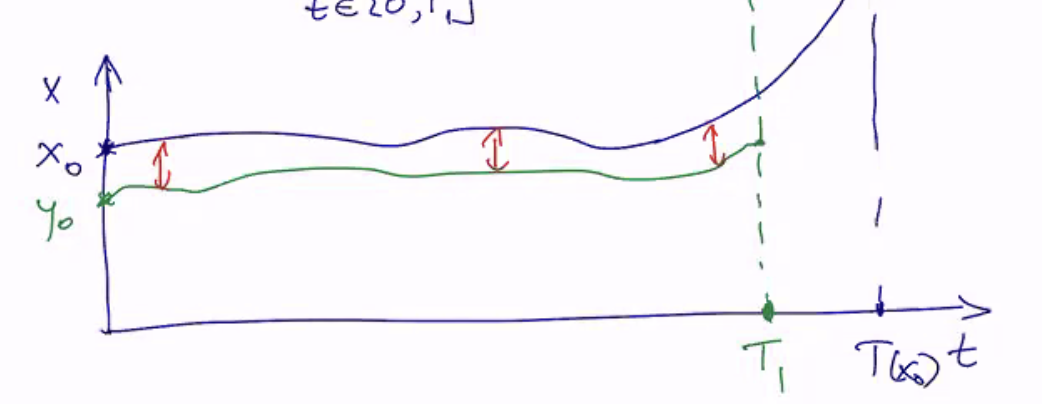
\includegraphics[scale=0.5]{localLipschitz.png}
\end{center}
\begin{thm}[Picard-Lindelof] Assume that $f$ is locally Lipschitz continuous.  Then the ODE is locally well-posed.
\end{thm}

\subsection{Contraction Principle}
We will use the "Contraction principle" - recall the following definitions:
\begin{definition}[Fixed-point Problem] Let $X$ be a Banach space,let $D \subset X$ be a closed subset of $X$, and let $F : D \rightarrow D$. Question: Can we solve the equation $F(u) = u$ where $u \in D$.
\end{definition}
\begin{definition}[Contraction] $$\|F(u) - F(v)\|_X \le L\|u - v\|,$$
where $L < 1$.
\end{definition}
If $F$ is a contraction, then it has a unique fixed point.  The existence proof follows an iterative construction: start with an arbitrary element $u_0 \in D$ and define $u_{n+1} = F(u_n)$.  We would show $\{u_n\}$ is a Cauchy sequence, so it converges.

We now prove the theorem.  We have $x' = f(x), x(0) = x_0$, so 
$$x(t) = x_0 + \int_{0}^t f(x(s))ds, t \in [0, T].$$
We choose $X = C[0, T; \R^n]$, $F(x)(t) = x_0 + \int_{0}^t f(x(s))ds.$ Then $x$ solves the ODE in $(0, T)$ if $F(x) = x$.
\begin{center}
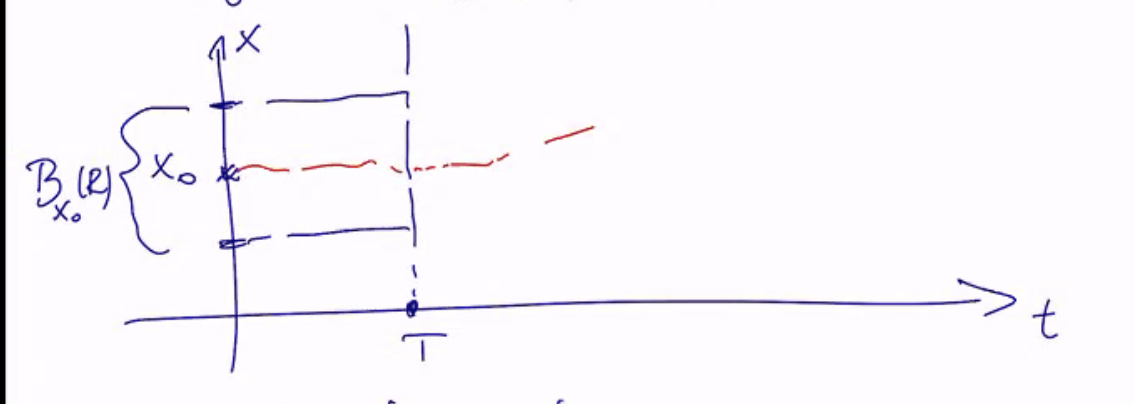
\includegraphics[scale=0.5]{ball.png}
\end{center}
We have to choose $R, T$.  Then
$$D = \{x \in X : \|x - x_0 \|_X \le R\}.$$

Let $R = |x_0|$.  Next, we choose $T$ so that $F : D \rightarrow D$ is Lipschitz.  For $F: D \rightarrow D$, we estimate the size of $F(x) - x_0$.
\begin{align*}
F(x)(t) - x_0| &= \left |\int_0^t f(x(s))ds\right | \\
&\le \left |\int_0^t f(x_0(s))ds\right | + \left | \int_0^t f(x) - f(x_0) ds \right | \\
&\le T |f(x_0)| + CT\|x - x_0\|_X  \\
\end{align*}
Hence,
$$\|F(x) - x_0\| \le T(|f(x_0)| + CR).$$
Thus, we choose $T$ such that $T(|f(x_0)| + CR) \le R$.

Now look at differences: For $x, y \in D$,
\begin{align*}
|F(x)(t) - F(y)(t)| &\le \int_{0}^t |f(x(s)) - f(y(s))| ds\\
&\le T C\sup_{s \in [0, T]} |x(s) - y(s)| \\
\end{align*}
thus,
$$\|F(x) - F(y)\|_X \le CT \|x - y\|_X,$$
so we can choose $T$ so that $CT\|x-y \|_X < 1$.

By the contraction principle, there exists a unique solution $x \in D$.  

To prove uniqueness of a solution, we have to show that any solution has to stay in $D$, up to time $T$.

\begin{center}
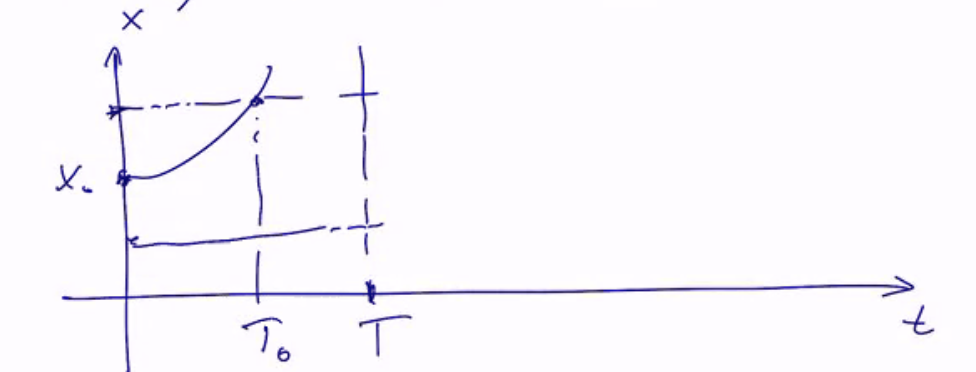
\includegraphics[scale=0.5]{unique.png}
\end{center}
Suppose a solution $\tilde{x}$ leave the ball before time $T$.  We repeat the above computation up to the exit time $T_0$.  Then, $T_0(|f(x_0) + CR|) < T$, since $T_0 < T$.  This is a contradiction since $T_0$ is the exit time.

\subsection{Bootstrap Argument}
Consider a bootstrap argument:  try to solve an equation and show that the solution $x$ satisfies some bound $\|x\|_T \le R$.  The difficulty is that a priori, we do not know any bound on $\|x\|_T$.  The solution:  make a bootstrap assumption, $\|x\|_T \le 2R$ and show that $\|x \|_T \le R$ under this assumption.  
\begin{center}
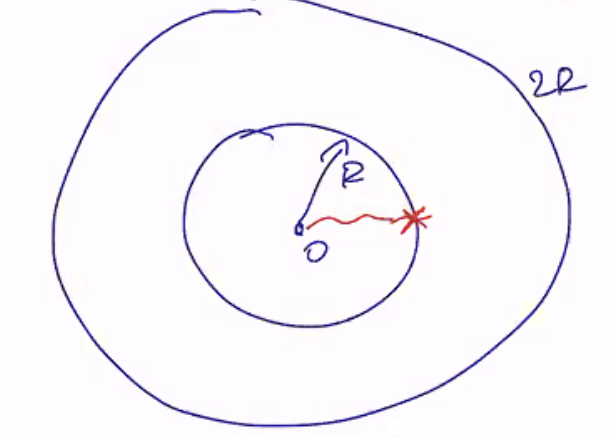
\includegraphics[scale=0.5]{bootstrap.png}
\end{center}

So far, we know uniqueness in $[0, T]$, where $T=T(x_0)$ given by the contraction argument.  We now show global uniqueness:  Suppose we have a solution $x_0$ with maximal lifespan $T_{max}(x_0)$.   Suppose $y$ is another solution.  We look at the maximal $T$ so that $x = y$ in $[0, T)$.  We now think of $T$ as the initial time.  We $x(T) = y(T)$ from continuity. Then, the solution is unique up to some time $T+T_0$, so $x = y$ in $[T, T+T_0]$, contradicting the maximality of $T$.  This is called a "continuity argument".

Next, we compare two solutions:  We have $x(0) = x_0, x: [0, T) \rightarrow R^n$.  We choose $T_1 < T$.  Then $x: [0, T_1] \rightarrow \R^n$.  We compare $x$ with a "nearby" solution $y(0) = y_0$ close to $x_0$.  We have$\|x\|_{X_{T_1}} \le R$ since we have continuity on a compact set.  We claim the following: if $|y_0 - x_0| < \epsilon$, then $x, y$ stay close.  We make a bootstrap assumption $\|y\|_{X_{T_1}} \le 2R$.  

$$\frac{d}{dt}|x-y|^2 = 2(x-y)(f(x) - f(y)) \le 2C|x-y|^2.$$

This is the \textit{Gronwall Inequality}.  It follows that $$|x-y|^2(t) \le e^{2ct}|x-y|^2(0) = e^{2ct}|x_0 - y_0|^2.$$
To close the bootstrap:
$$\|y\|_{X_{T_1}} \le \|x\|_{X_{T_1}} + \|x-y\|_{X_{T_1}} \le R + e^{cT_1}\|x_0 - y_0\| \le \frac{3R}{2},$$
which is better than the bootstrap assumption.
\end{document}
